\documentclass[1p]{elsarticle_modified}
%\bibliographystyle{elsarticle-num}

%\usepackage[colorlinks]{hyperref}
%\usepackage{abbrmath_seonhwa} %\Abb, \Ascr, \Acal ,\Abf, \Afrak
\usepackage{amsfonts}
\usepackage{amssymb}
\usepackage{amsmath}
\usepackage{amsthm}
\usepackage{scalefnt}
\usepackage{amsbsy}
\usepackage{kotex}
\usepackage{caption}
\usepackage{subfig}
\usepackage{color}
\usepackage{graphicx}
\usepackage{xcolor} %% white, black, red, green, blue, cyan, magenta, yellow
\usepackage{float}
\usepackage{setspace}
\usepackage{hyperref}

\usepackage{tikz}
\usetikzlibrary{arrows}

\usepackage{multirow}
\usepackage{array} % fixed length table
\usepackage{hhline}

%%%%%%%%%%%%%%%%%%%%%
\makeatletter
\renewcommand*\env@matrix[1][\arraystretch]{%
	\edef\arraystretch{#1}%
	\hskip -\arraycolsep
	\let\@ifnextchar\new@ifnextchar
	\array{*\c@MaxMatrixCols c}}
\makeatother %https://tex.stackexchange.com/questions/14071/how-can-i-increase-the-line-spacing-in-a-matrix
%%%%%%%%%%%%%%%

\usepackage[normalem]{ulem}

\newcommand{\msout}[1]{\ifmmode\text{\sout{\ensuremath{#1}}}\else\sout{#1}\fi}
%SOURCE: \msout is \stkout macro in https://tex.stackexchange.com/questions/20609/strikeout-in-math-mode

\newcommand{\cancel}[1]{
	\ifmmode
	{\color{red}\msout{#1}}
	\else
	{\color{red}\sout{#1}}
	\fi
}

\newcommand{\add}[1]{
	{\color{blue}\uwave{#1}}
}

\newcommand{\replace}[2]{
	\ifmmode
	{\color{red}\msout{#1}}{\color{blue}\uwave{#2}}
	\else
	{\color{red}\sout{#1}}{\color{blue}\uwave{#2}}
	\fi
}

\newcommand{\Sol}{\mathcal{S}} %segment
\newcommand{\D}{D} %diagram
\newcommand{\A}{\mathcal{A}} %arc


%%%%%%%%%%%%%%%%%%%%%%%%%%%%%5 test

\def\sl{\operatorname{\textup{SL}}(2,\Cbb)}
\def\psl{\operatorname{\textup{PSL}}(2,\Cbb)}
\def\quan{\mkern 1mu \triangleright \mkern 1mu}

\theoremstyle{definition}
\newtheorem{thm}{Theorem}[section]
\newtheorem{prop}[thm]{Proposition}
\newtheorem{lem}[thm]{Lemma}
\newtheorem{ques}[thm]{Question}
\newtheorem{cor}[thm]{Corollary}
\newtheorem{defn}[thm]{Definition}
\newtheorem{exam}[thm]{Example}
\newtheorem{rmk}[thm]{Remark}
\newtheorem{alg}[thm]{Algorithm}

\newcommand{\I}{\sqrt{-1}}
\begin{document}

%\begin{frontmatter}
%
%\title{Boundary parabolic representations of knots up to 8 crossings}
%
%%% Group authors per affiliation:
%\author{Yunhi Cho} 
%\address{Department of Mathematics, University of Seoul, Seoul, Korea}
%\ead{yhcho@uos.ac.kr}
%
%
%\author{Seonhwa Kim} %\fnref{s_kim}}
%\address{Center for Geometry and Physics, Institute for Basic Science, Pohang, 37673, Korea}
%\ead{ryeona17@ibs.re.kr}
%
%\author{Hyuk Kim}
%\address{Department of Mathematical Sciences, Seoul National University, Seoul 08826, Korea}
%\ead{hyukkim@snu.ac.kr}
%
%\author{Seokbeom Yoon}
%\address{Department of Mathematical Sciences, Seoul National University, Seoul, 08826,  Korea}
%\ead{sbyoon15@snu.ac.kr}
%
%\begin{abstract}
%We find all boundary parabolic representation of knots up to 8 crossings.
%
%\end{abstract}
%\begin{keyword}
%    \MSC[2010] 57M25 
%\end{keyword}
%
%\end{frontmatter}

%\linenumbers
%\tableofcontents
%
\newcommand\colored[1]{\textcolor{white}{\rule[-0.35ex]{0.8em}{1.4ex}}\kern-0.8em\color{red} #1}%
%\newcommand\colored[1]{\textcolor{white}{ #1}\kern-2.17ex	\textcolor{white}{ #1}\kern-1.81ex	\textcolor{white}{ #1}\kern-2.15ex\color{red}#1	}

{\Large $\underline{9_{22}~(K9a_{2})}$}

\setlength{\tabcolsep}{10pt}
\renewcommand{\arraystretch}{1.6}
\vspace{1cm}\begin{tabular}{m{100pt}>{\centering\arraybackslash}m{274pt}}
\multirow{5}{120pt}{
	\centering
	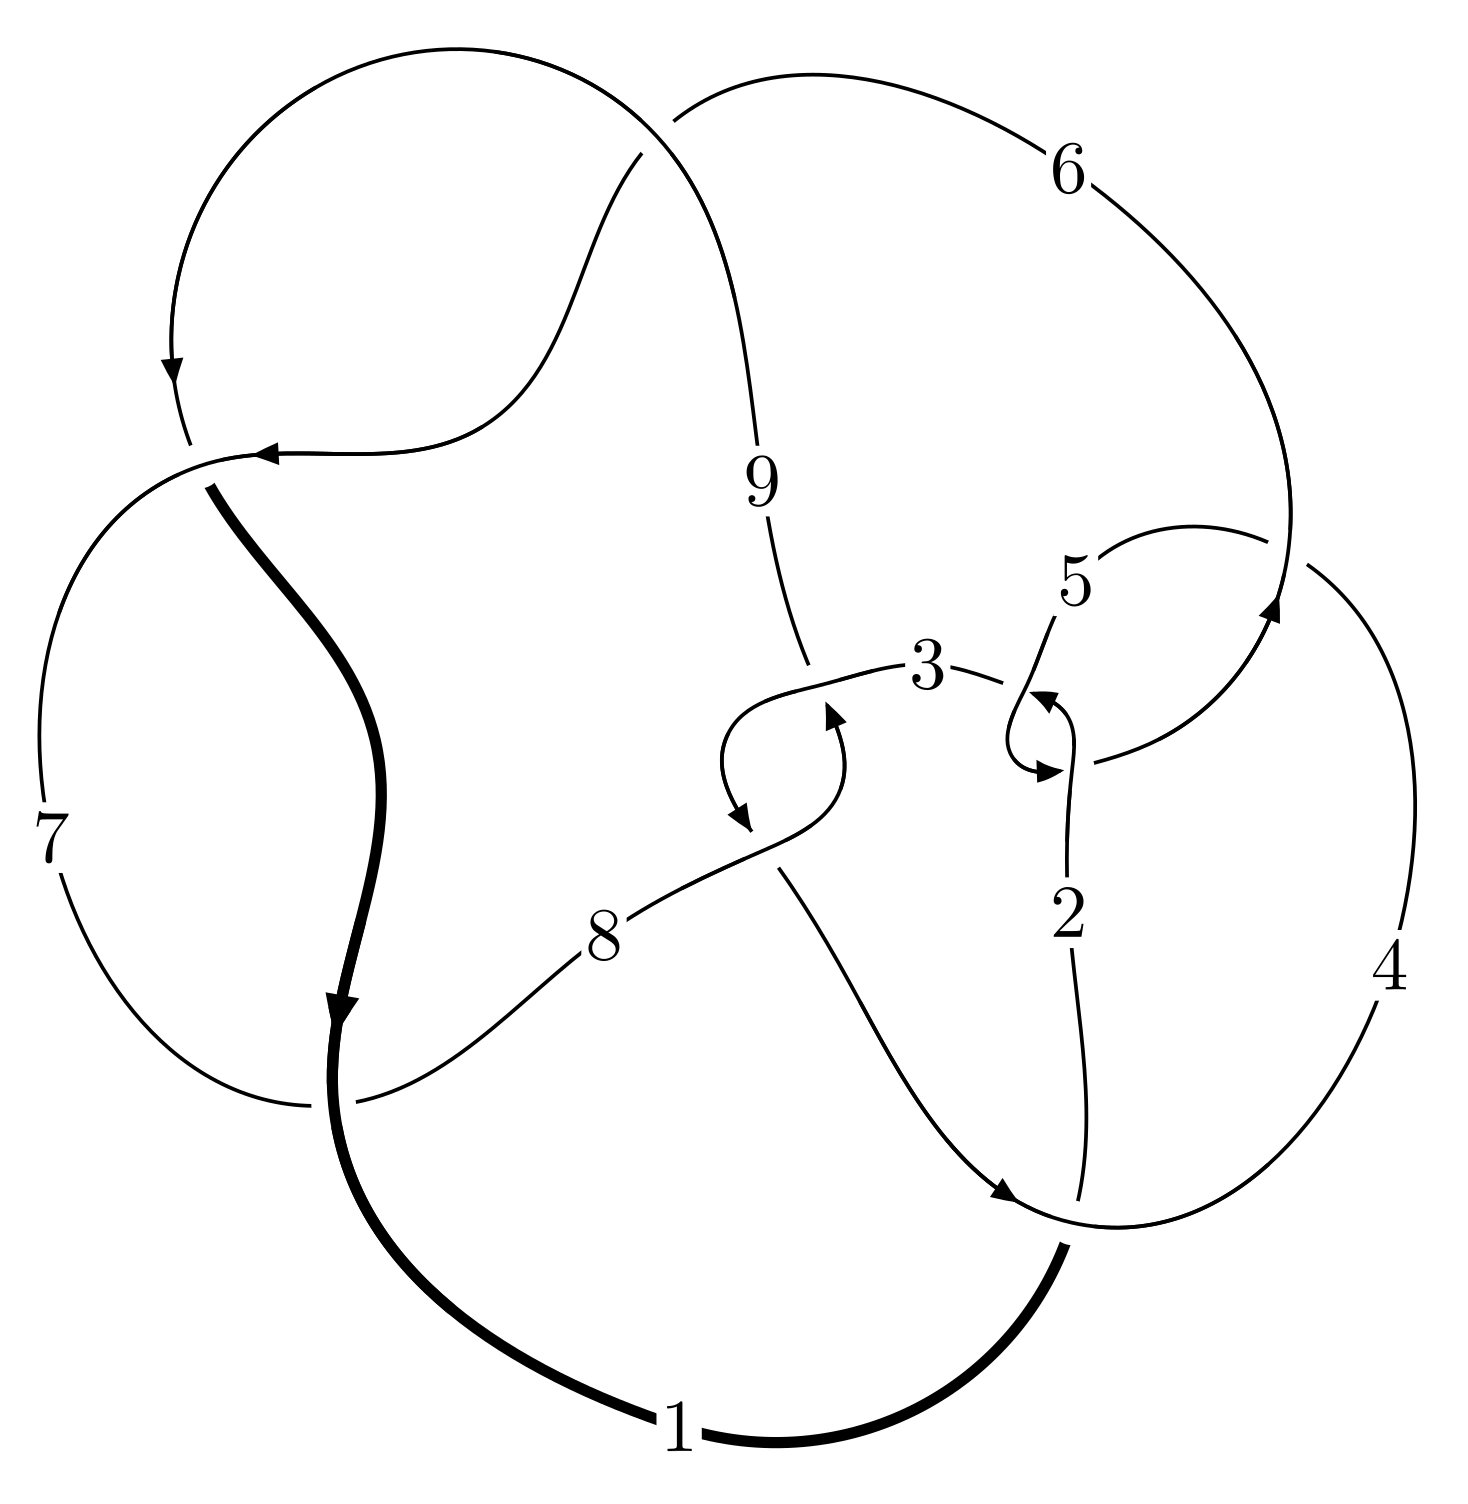
\includegraphics[width=112pt]{../../../GIT/diagram.site/Diagrams/png/57_9_22.png}\\
\ \ \ A knot diagram\footnotemark}&
\allowdisplaybreaks
\textbf{Linearized knot diagam} \\
\cline{2-2}
 &
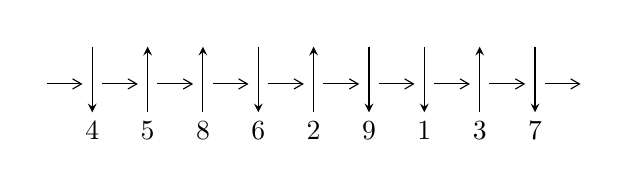
\begin{tikzpicture}[x=20pt, y=17pt]
	% nodes
	\node (C0) at (0, 0) {};
	\node (C1) at (1, 0) {};
	\node (C1U) at (1, +1) {};
	\node (C1D) at (1, -1) {4};

	\node (C2) at (2, 0) {};
	\node (C2U) at (2, +1) {};
	\node (C2D) at (2, -1) {5};

	\node (C3) at (3, 0) {};
	\node (C3U) at (3, +1) {};
	\node (C3D) at (3, -1) {8};

	\node (C4) at (4, 0) {};
	\node (C4U) at (4, +1) {};
	\node (C4D) at (4, -1) {6};

	\node (C5) at (5, 0) {};
	\node (C5U) at (5, +1) {};
	\node (C5D) at (5, -1) {2};

	\node (C6) at (6, 0) {};
	\node (C6U) at (6, +1) {};
	\node (C6D) at (6, -1) {9};

	\node (C7) at (7, 0) {};
	\node (C7U) at (7, +1) {};
	\node (C7D) at (7, -1) {1};

	\node (C8) at (8, 0) {};
	\node (C8U) at (8, +1) {};
	\node (C8D) at (8, -1) {3};

	\node (C9) at (9, 0) {};
	\node (C9U) at (9, +1) {};
	\node (C9D) at (9, -1) {7};
	\node (C10) at (10, 0) {};

	% arrows
	\draw[->,>={angle 60}]
	(C0) edge (C1) (C1) edge (C2) (C2) edge (C3) (C3) edge (C4) (C4) edge (C5) (C5) edge (C6) (C6) edge (C7) (C7) edge (C8) (C8) edge (C9) (C9) edge (C10) ;	\draw[->,>=stealth]
	(C1U) edge (C1D) (C2D) edge (C2U) (C3D) edge (C3U) (C4U) edge (C4D) (C5D) edge (C5U) (C6U) edge (C6D) (C7U) edge (C7D) (C8D) edge (C8U) (C9U) edge (C9D) ;
	\end{tikzpicture} \\
\hhline{~~} \\& 
\textbf{Solving Sequence} \\ \cline{2-2} 
 &
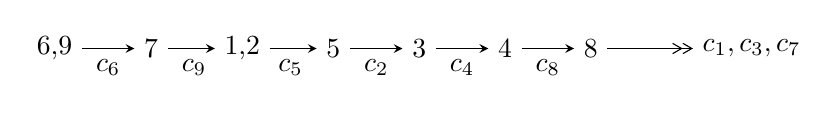
\begin{tikzpicture}[x=31pt, y=7pt]
	% node
	\node (A0) at (-1/8, 0) {6,9};
	\node (A1) at (1, 0) {7};
	\node (A2) at (33/16, 0) {1,2};
	\node (A3) at (25/8, 0) {5};
	\node (A4) at (33/8, 0) {3};
	\node (A5) at (41/8, 0) {4};
	\node (A6) at (49/8, 0) {8};
	\node (C1) at (1/2, -1) {$c_{6}$};
	\node (C2) at (3/2, -1) {$c_{9}$};
	\node (C3) at (21/8, -1) {$c_{5}$};
	\node (C4) at (29/8, -1) {$c_{2}$};
	\node (C5) at (37/8, -1) {$c_{4}$};
	\node (C6) at (45/8, -1) {$c_{8}$};
	\node (A7) at (8, 0) {$c_{1},c_{3},c_{7}$};

	% edge
	\draw[->,>=stealth]	
	(A0) edge (A1) (A1) edge (A2) (A2) edge (A3) (A3) edge (A4) (A4) edge (A5) (A5) edge (A6) ;
	\draw[->>,>={angle 60}]	
	(A6) edge (A7);
\end{tikzpicture} \\ 

\end{tabular} \\

\footnotetext{
The image of knot diagram is generated by the software ``\textbf{Draw programme}" developed by Andrew Bartholomew(\url{http://www.layer8.co.uk/maths/draw/index.htm\#Running-draw}), where we modified some parts for our purpose(\url{https://github.com/CATsTAILs/LinksPainter}).
}\phantom \\ \newline 
\centering \textbf{Ideals for irreducible components\footnotemark of $X_{\text{par}}$} 
 
\begin{align*}
I^u_{1}&=\langle 
- u^{22}-2 u^{21}+\cdots+2 b+1,\;- u^6+3 u^4-2 u^3-2 u^2+a+4 u-1,\;u^{23}+3 u^{22}+\cdots- u-1\rangle \\
I^u_{2}&=\langle 
b^2- b+1,\;a+1,\;u-1\rangle \\
\\
\end{align*}
\raggedright * 2 irreducible components of $\dim_{\mathbb{C}}=0$, with total 25 representations.\\
\footnotetext{All coefficients of polynomials are rational numbers. But the coefficients are sometimes approximated in decimal forms when there is not enough margin.}
\newpage
\renewcommand{\arraystretch}{1}
\centering \section*{I. $I^u_{1}= \langle - u^{22}-2 u^{21}+\cdots+2 b+1,\;- u^6+3 u^4-2 u^3-2 u^2+a+4 u-1,\;u^{23}+3 u^{22}+\cdots- u-1 \rangle$}
\flushleft \textbf{(i) Arc colorings}\\
\begin{tabular}{m{7pt} m{180pt} m{7pt} m{180pt} }
\flushright $a_{6}=$&$\begin{pmatrix}1\\0\end{pmatrix}$ \\
\flushright $a_{9}=$&$\begin{pmatrix}0\\u\end{pmatrix}$ \\
\flushright $a_{7}=$&$\begin{pmatrix}1\\u^2\end{pmatrix}$ \\
\flushright $a_{1}=$&$\begin{pmatrix}- u\\- u^3+u\end{pmatrix}$ \\
\flushright $a_{2}=$&$\begin{pmatrix}u^6-3 u^4+2 u^3+2 u^2-4 u+1\\\frac{1}{2} u^{22}+u^{21}+\cdots+2 u^2-\frac{1}{2}\end{pmatrix}$ \\
\flushright $a_{5}=$&$\begin{pmatrix}\frac{3}{2} u^{22}+3 u^{21}+\cdots-2 u^2-\frac{1}{2}\\-\frac{5}{2} u^{22}-4 u^{21}+\cdots+u+\frac{3}{2}\end{pmatrix}$ \\
\flushright $a_{3}=$&$\begin{pmatrix}-2 u^{22}-3 u^{21}+\cdots- u+1\\\frac{3}{2} u^{22}+2 u^{21}+\cdots- u^2-\frac{1}{2}\end{pmatrix}$ \\
\flushright $a_{4}=$&$\begin{pmatrix}- u^{22}- u^{21}+\cdots+u+1\\-\frac{5}{2} u^{22}-4 u^{21}+\cdots+u+\frac{3}{2}\end{pmatrix}$ \\
\flushright $a_{8}=$&$\begin{pmatrix}- u^2+1\\- u^4+2 u^2\end{pmatrix}$\\ \flushright $a_{8}=$&$\begin{pmatrix}- u^2+1\\- u^4+2 u^2\end{pmatrix}$\\&\end{tabular}
\flushleft \textbf{(ii) Obstruction class $= -1$}\\~\\
\flushleft \textbf{(iii) Cusp Shapes $= 3 u^{22}+3 u^{21}-32 u^{20}-19 u^{19}+155 u^{18}+15 u^{17}-432 u^{16}+194 u^{15}+690 u^{14}-758 u^{13}-450 u^{12}+1221 u^{11}-359 u^{10}-839 u^9+820 u^8-2 u^7-401 u^6+227 u^5-22 u^4-21 u^3+u^2+u$}\\~\\
\newpage\renewcommand{\arraystretch}{1}
\flushleft \textbf{(iv) u-Polynomials at the component}\newline \\
\begin{tabular}{m{50pt}|m{274pt}}
Crossings & \hspace{64pt}u-Polynomials at each crossing \\
\hline $$\begin{aligned}c_{1}\end{aligned}$$&$\begin{aligned}
&u^{23}-2 u^{22}+\cdots+18 u-9
\end{aligned}$\\
\hline $$\begin{aligned}c_{2},c_{5}\end{aligned}$$&$\begin{aligned}
&u^{23}+2 u^{22}+\cdots-2 u-1
\end{aligned}$\\
\hline $$\begin{aligned}c_{3},c_{8}\end{aligned}$$&$\begin{aligned}
&u^{23}- u^{22}+\cdots+8 u+4
\end{aligned}$\\
\hline $$\begin{aligned}c_{4}\end{aligned}$$&$\begin{aligned}
&u^{23}+12 u^{22}+\cdots-2 u-1
\end{aligned}$\\
\hline $$\begin{aligned}c_{6},c_{7},c_{9}\end{aligned}$$&$\begin{aligned}
&u^{23}-3 u^{22}+\cdots- u+1
\end{aligned}$\\
\hline
\end{tabular}\\~\\
\newpage\renewcommand{\arraystretch}{1}
\flushleft \textbf{(v) Riley Polynomials at the component}\newline \\
\begin{tabular}{m{50pt}|m{274pt}}
Crossings & \hspace{64pt}Riley Polynomials at each crossing \\
\hline $$\begin{aligned}c_{1}\end{aligned}$$&$\begin{aligned}
&y^{23}-12 y^{22}+\cdots-450 y-81
\end{aligned}$\\
\hline $$\begin{aligned}c_{2},c_{5}\end{aligned}$$&$\begin{aligned}
&y^{23}+12 y^{22}+\cdots-2 y-1
\end{aligned}$\\
\hline $$\begin{aligned}c_{3},c_{8}\end{aligned}$$&$\begin{aligned}
&y^{23}+15 y^{22}+\cdots-40 y-16
\end{aligned}$\\
\hline $$\begin{aligned}c_{4}\end{aligned}$$&$\begin{aligned}
&y^{23}+24 y^{21}+\cdots+10 y-1
\end{aligned}$\\
\hline $$\begin{aligned}c_{6},c_{7},c_{9}\end{aligned}$$&$\begin{aligned}
&y^{23}-23 y^{22}+\cdots-7 y-1
\end{aligned}$\\
\hline
\end{tabular}\\~\\
\newpage\flushleft \textbf{(vi) Complex Volumes and Cusp Shapes}
$$\begin{array}{c|c|c}  
\text{Solutions to }I^u_{1}& \I (\text{vol} + \sqrt{-1}CS) & \text{Cusp shape}\\
 \hline 
\begin{aligned}
u &= \phantom{-}0.696926 + 0.678563 I \\
a &= -0.371551 - 0.457637 I \\
b &= \phantom{-}0.386982 + 1.120880 I\end{aligned}
 & -4.15124 + 1.33135 I & -7.15950 - 0.67575 I \\ \hline\begin{aligned}
u &= \phantom{-}0.696926 - 0.678563 I \\
a &= -0.371551 + 0.457637 I \\
b &= \phantom{-}0.386982 - 1.120880 I\end{aligned}
 & -4.15124 - 1.33135 I & -7.15950 + 0.67575 I \\ \hline\begin{aligned}
u &= \phantom{-}1.026370 + 0.230969 I \\
a &= -1.271710 - 0.069358 I \\
b &= \phantom{-}0.179248 - 0.701899 I\end{aligned}
 & -2.10210 - 0.88878 I & -6.39291 - 0.92577 I \\ \hline\begin{aligned}
u &= \phantom{-}1.026370 - 0.230969 I \\
a &= -1.271710 + 0.069358 I \\
b &= \phantom{-}0.179248 + 0.701899 I\end{aligned}
 & -2.10210 + 0.88878 I & -6.39291 + 0.92577 I \\ \hline\begin{aligned}
u &= \phantom{-}0.443194 + 0.830987 I \\
a &= -1.84438 + 0.30451 I \\
b &= \phantom{-}0.501837 - 1.137100 I\end{aligned}
 & -3.32060 - 6.47771 I & -4.77780 + 6.52194 I \\ \hline\begin{aligned}
u &= \phantom{-}0.443194 - 0.830987 I \\
a &= -1.84438 - 0.30451 I \\
b &= \phantom{-}0.501837 + 1.137100 I\end{aligned}
 & -3.32060 + 6.47771 I & -4.77780 - 6.52194 I \\ \hline\begin{aligned}
u &= \phantom{-}0.411789 + 0.657552 I \\
a &= -1.215710 - 0.639418 I \\
b &= \phantom{-}0.657802 + 0.201077 I\end{aligned}
 & -0.66432 - 2.00215 I & -1.23588 + 3.62705 I \\ \hline\begin{aligned}
u &= \phantom{-}0.411789 - 0.657552 I \\
a &= -1.215710 + 0.639418 I \\
b &= \phantom{-}0.657802 - 0.201077 I\end{aligned}
 & -0.66432 + 2.00215 I & -1.23588 - 3.62705 I \\ \hline\begin{aligned}
u &= \phantom{-}1.31043\phantom{ +0.000000I} \\
a &= -0.0893487\phantom{ +0.000000I} \\
b &= -0.616508\phantom{ +0.000000I}\end{aligned}
 & -2.78711\phantom{ +0.000000I} & -2.32390\phantom{ +0.000000I} \\ \hline\begin{aligned}
u &= -1.349890 + 0.050765 I \\
a &= \phantom{-}1.185670 + 0.215112 I \\
b &= -0.730473 - 0.812317 I\end{aligned}
 & -3.41052 + 2.74438 I & -6.00137 - 3.42075 I\\
 \hline 
 \end{array}$$\newpage$$\begin{array}{c|c|c}  
\text{Solutions to }I^u_{1}& \I (\text{vol} + \sqrt{-1}CS) & \text{Cusp shape}\\
 \hline 
\begin{aligned}
u &= -1.349890 - 0.050765 I \\
a &= \phantom{-}1.185670 - 0.215112 I \\
b &= -0.730473 + 0.812317 I\end{aligned}
 & -3.41052 - 2.74438 I & -6.00137 + 3.42075 I \\ \hline\begin{aligned}
u &= \phantom{-}1.42968 + 0.09520 I \\
a &= \phantom{-}0.89149 + 1.36719 I \\
b &= -0.449028 + 1.143790 I\end{aligned}
 & -5.84331 - 3.99588 I & -6.60901 + 3.49800 I \\ \hline\begin{aligned}
u &= \phantom{-}1.42968 - 0.09520 I \\
a &= \phantom{-}0.89149 - 1.36719 I \\
b &= -0.449028 - 1.143790 I\end{aligned}
 & -5.84331 + 3.99588 I & -6.60901 - 3.49800 I \\ \hline\begin{aligned}
u &= -1.48042 + 0.24817 I \\
a &= -0.537692 + 0.556573 I \\
b &= \phantom{-}0.868940 - 0.243856 I\end{aligned}
 & -6.80889 + 5.35900 I & -4.49542 - 3.06793 I \\ \hline\begin{aligned}
u &= -1.48042 - 0.24817 I \\
a &= -0.537692 - 0.556573 I \\
b &= \phantom{-}0.868940 + 0.243856 I\end{aligned}
 & -6.80889 - 5.35900 I & -4.49542 + 3.06793 I \\ \hline\begin{aligned}
u &= -1.51052 + 0.30516 I \\
a &= -1.54699 + 0.69863 I \\
b &= \phantom{-}0.565955 + 1.190510 I\end{aligned}
 & -9.6533 + 10.6207 I & -7.02627 - 6.45650 I \\ \hline\begin{aligned}
u &= -1.51052 - 0.30516 I \\
a &= -1.54699 - 0.69863 I \\
b &= \phantom{-}0.565955 - 1.190510 I\end{aligned}
 & -9.6533 - 10.6207 I & -7.02627 + 6.45650 I \\ \hline\begin{aligned}
u &= -1.55320 + 0.17815 I \\
a &= -0.002579 - 0.587301 I \\
b &= \phantom{-}0.282827 - 1.245840 I\end{aligned}
 & -11.61980 + 1.64388 I & -9.30470 - 0.40272 I \\ \hline\begin{aligned}
u &= -1.55320 - 0.17815 I \\
a &= -0.002579 + 0.587301 I \\
b &= \phantom{-}0.282827 + 1.245840 I\end{aligned}
 & -11.61980 - 1.64388 I & -9.30470 + 0.40272 I \\ \hline\begin{aligned}
u &= \phantom{-}0.008249 + 0.425434 I \\
a &= \phantom{-}0.49224 - 1.83322 I \\
b &= -0.476560 + 0.630579 I\end{aligned}
 & \phantom{-}0.71923 - 1.37448 I & \phantom{-}2.70178 + 4.35124 I\\
 \hline 
 \end{array}$$\newpage$$\begin{array}{c|c|c}  
\text{Solutions to }I^u_{1}& \I (\text{vol} + \sqrt{-1}CS) & \text{Cusp shape}\\
 \hline 
\begin{aligned}
u &= \phantom{-}0.008249 - 0.425434 I \\
a &= \phantom{-}0.49224 + 1.83322 I \\
b &= -0.476560 - 0.630579 I\end{aligned}
 & \phantom{-}0.71923 + 1.37448 I & \phantom{-}2.70178 - 4.35124 I \\ \hline\begin{aligned}
u &= -0.277376 + 0.277332 I \\
a &= \phantom{-}2.26589 - 1.32800 I \\
b &= -0.479277 - 0.962679 I\end{aligned}
 & -0.27712 + 2.59653 I & \phantom{-}1.46303 - 3.78636 I \\ \hline\begin{aligned}
u &= -0.277376 - 0.277332 I \\
a &= \phantom{-}2.26589 + 1.32800 I \\
b &= -0.479277 + 0.962679 I\end{aligned}
 & -0.27712 - 2.59653 I & \phantom{-}1.46303 + 3.78636 I\\
 \hline 
 \end{array}$$\newpage\newpage\renewcommand{\arraystretch}{1}
\centering \section*{II. $I^u_{2}= \langle b^2- b+1,\;a+1,\;u-1 \rangle$}
\flushleft \textbf{(i) Arc colorings}\\
\begin{tabular}{m{7pt} m{180pt} m{7pt} m{180pt} }
\flushright $a_{6}=$&$\begin{pmatrix}1\\0\end{pmatrix}$ \\
\flushright $a_{9}=$&$\begin{pmatrix}0\\1\end{pmatrix}$ \\
\flushright $a_{7}=$&$\begin{pmatrix}1\\1\end{pmatrix}$ \\
\flushright $a_{1}=$&$\begin{pmatrix}-1\\0\end{pmatrix}$ \\
\flushright $a_{2}=$&$\begin{pmatrix}-1\\b\end{pmatrix}$ \\
\flushright $a_{5}=$&$\begin{pmatrix}- b+1\\b-1\end{pmatrix}$ \\
\flushright $a_{3}=$&$\begin{pmatrix}0\\b-1\end{pmatrix}$ \\
\flushright $a_{4}=$&$\begin{pmatrix}0\\b-1\end{pmatrix}$ \\
\flushright $a_{8}=$&$\begin{pmatrix}0\\1\end{pmatrix}$\\ \flushright $a_{8}=$&$\begin{pmatrix}0\\1\end{pmatrix}$\\&\end{tabular}
\flushleft \textbf{(ii) Obstruction class $= 1$}\\~\\
\flushleft \textbf{(iii) Cusp Shapes $= -4 b-1$}\\~\\
\newpage\renewcommand{\arraystretch}{1}
\flushleft \textbf{(iv) u-Polynomials at the component}\newline \\
\begin{tabular}{m{50pt}|m{274pt}}
Crossings & \hspace{64pt}u-Polynomials at each crossing \\
\hline $$\begin{aligned}c_{1},c_{4},c_{5}\end{aligned}$$&$\begin{aligned}
&u^2- u+1
\end{aligned}$\\
\hline $$\begin{aligned}c_{2}\end{aligned}$$&$\begin{aligned}
&u^2+u+1
\end{aligned}$\\
\hline $$\begin{aligned}c_{3},c_{8}\end{aligned}$$&$\begin{aligned}
&u^2
\end{aligned}$\\
\hline $$\begin{aligned}c_{6},c_{7}\end{aligned}$$&$\begin{aligned}
&(u-1)^2
\end{aligned}$\\
\hline $$\begin{aligned}c_{9}\end{aligned}$$&$\begin{aligned}
&(u+1)^2
\end{aligned}$\\
\hline
\end{tabular}\\~\\
\newpage\renewcommand{\arraystretch}{1}
\flushleft \textbf{(v) Riley Polynomials at the component}\newline \\
\begin{tabular}{m{50pt}|m{274pt}}
Crossings & \hspace{64pt}Riley Polynomials at each crossing \\
\hline $$\begin{aligned}c_{1},c_{2},c_{4}\\c_{5}\end{aligned}$$&$\begin{aligned}
&y^2+y+1
\end{aligned}$\\
\hline $$\begin{aligned}c_{3},c_{8}\end{aligned}$$&$\begin{aligned}
&y^2
\end{aligned}$\\
\hline $$\begin{aligned}c_{6},c_{7},c_{9}\end{aligned}$$&$\begin{aligned}
&(y-1)^2
\end{aligned}$\\
\hline
\end{tabular}\\~\\
\newpage\flushleft \textbf{(vi) Complex Volumes and Cusp Shapes}
$$\begin{array}{c|c|c}  
\text{Solutions to }I^u_{2}& \I (\text{vol} + \sqrt{-1}CS) & \text{Cusp shape}\\
 \hline 
\begin{aligned}
u &= \phantom{-}1.00000\phantom{ +0.000000I} \\
a &= -1.00000\phantom{ +0.000000I} \\
b &= \phantom{-}0.500000 + 0.866025 I\end{aligned}
 & -1.64493 + 2.02988 I & -3.00000 - 3.46410 I \\ \hline\begin{aligned}
u &= \phantom{-}1.00000\phantom{ +0.000000I} \\
a &= -1.00000\phantom{ +0.000000I} \\
b &= \phantom{-}0.500000 - 0.866025 I\end{aligned}
 & -1.64493 - 2.02988 I & -3.00000 + 3.46410 I\\
 \hline 
 \end{array}$$\newpage
\newpage\renewcommand{\arraystretch}{1}
\centering \section*{ III. u-Polynomials}
\begin{tabular}{m{50pt}|m{274pt}}
Crossings & \hspace{64pt}u-Polynomials at each crossing \\
\hline $$\begin{aligned}c_{1}\end{aligned}$$&$\begin{aligned}
&(u^2- u+1)(u^{23}-2 u^{22}+\cdots+18 u-9)
\end{aligned}$\\
\hline $$\begin{aligned}c_{2}\end{aligned}$$&$\begin{aligned}
&(u^2+u+1)(u^{23}+2 u^{22}+\cdots-2 u-1)
\end{aligned}$\\
\hline $$\begin{aligned}c_{3},c_{8}\end{aligned}$$&$\begin{aligned}
&u^2(u^{23}- u^{22}+\cdots+8 u+4)
\end{aligned}$\\
\hline $$\begin{aligned}c_{4}\end{aligned}$$&$\begin{aligned}
&(u^2- u+1)(u^{23}+12 u^{22}+\cdots-2 u-1)
\end{aligned}$\\
\hline $$\begin{aligned}c_{5}\end{aligned}$$&$\begin{aligned}
&(u^2- u+1)(u^{23}+2 u^{22}+\cdots-2 u-1)
\end{aligned}$\\
\hline $$\begin{aligned}c_{6},c_{7}\end{aligned}$$&$\begin{aligned}
&((u-1)^2)(u^{23}-3 u^{22}+\cdots- u+1)
\end{aligned}$\\
\hline $$\begin{aligned}c_{9}\end{aligned}$$&$\begin{aligned}
&((u+1)^2)(u^{23}-3 u^{22}+\cdots- u+1)
\end{aligned}$\\
\hline
\end{tabular}\newpage\renewcommand{\arraystretch}{1}
\centering \section*{ IV. Riley Polynomials}
\begin{tabular}{m{50pt}|m{274pt}}
Crossings & \hspace{64pt}Riley Polynomials at each crossing \\
\hline $$\begin{aligned}c_{1}\end{aligned}$$&$\begin{aligned}
&(y^2+y+1)(y^{23}-12 y^{22}+\cdots-450 y-81)
\end{aligned}$\\
\hline $$\begin{aligned}c_{2},c_{5}\end{aligned}$$&$\begin{aligned}
&(y^2+y+1)(y^{23}+12 y^{22}+\cdots-2 y-1)
\end{aligned}$\\
\hline $$\begin{aligned}c_{3},c_{8}\end{aligned}$$&$\begin{aligned}
&y^2(y^{23}+15 y^{22}+\cdots-40 y-16)
\end{aligned}$\\
\hline $$\begin{aligned}c_{4}\end{aligned}$$&$\begin{aligned}
&(y^2+y+1)(y^{23}+24 y^{21}+\cdots+10 y-1)
\end{aligned}$\\
\hline $$\begin{aligned}c_{6},c_{7},c_{9}\end{aligned}$$&$\begin{aligned}
&((y-1)^2)(y^{23}-23 y^{22}+\cdots-7 y-1)
\end{aligned}$\\
\hline
\end{tabular}
\vskip 2pc
\end{document}